\chapter{Discussion}
Biases on models from confounding elements have been widely reported in machine learning
\cite{DeConstructing_Bias_on_Skin_Lesion_Datasets_2019, Towards_Explainable_Classifiers_Using_the_Counterfactual_Approach_2019, debias-not-so-fast, interps-are-useful}.

The initial goal of this project was to look into methods to not use ruler presence in the
classification of lesions.
To be able to investigate the phenomenon, the plan was to:
\begin{enumerate}
    \item Train a model that performs fairly well compared to the state-of-the-art \label{item:train-model}
    \item Show that the model is using the presence of ruler in its predictions \label{item:biased-ruler}
    \item Modify the model to remove the bias
    \item Rerun the argument as in step \ref{item:biased-ruler} and show that the model is no longer biased
\end{enumerate}
Step \ref{item:train-model} went fairly easy, especially because the dataset is well researched,
so, another model could be used for inspiration \cite{kaggle-97-model}.

When reaching step \ref{item:biased-ruler}, the results didn't go quite as expected.
Even though it had been argued in previous papers that models were doing exactly this
\cite{debias-not-so-fast,interps-are-useful}, I was unable to replicate their results,
to a degree, that convinced me that the model was indeed using the rulers.
This changed the focus of the project from removing biased predictions to instead investigating
if there were any biases at all.
In the following, we will go through the experiments made in Section \ref{sec:testing-the-hypothesis} and
examine the results in this light: Do they seem to indicate that the model is using the rulers?

The discussion will be divided into a part where the results of the analysis in Section \ref{sec:testing-the-hypothesis}
are examined, and a part where we will discuss the results of the project in its entirety.
It will be finished up with what obvious further research that could be done following up this project.

\section{Discussion of analysis}
\subsection{Saliency maps}
In Section \ref{sec:prediction-saliency-map} we investigated the saliency maps of the model predictions.
Previously, other researchers had shown that the rulers would be indicated clearly on these maps \cite{interps-are-useful}.
Going through the same experiment with the model trained in this project, we found saliency maps that did not indicate anything clearly. 
(see Figure \ref{fig:interps-are-useful-saliency-maps} and \ref{fig:ruler_saliency_map}).
In some instances, the lesion was not even visible in the highlighted areas,
and in others it was, but not in a way where it was obviously using that specific element of the image.

In general, class-specific gradient based saliency maps are very prone to confirmation bias \cite{sanity-checks-for-saliency,Grns2020FaithfulSM}.
It is nothing more than the gradient on a very complicated function.
Conclude that just because the ruler is sometimes highlighted partly on the saliency map,
it must mean that the model is using it, seems like a stretch on its own.
Especially when considering the saliency maps from the model trained on segmented images (Figure 
\ref{fig:segmented_prediction_saliency_map}) that is highlighting the ruler to at least the same degree 
that the model trained on the entire dataset is.
We know for sure, that the model trained on the segmented dataset is not using the rulers,
as it has never seen a ruler during training.
It is unclear exactly what knowledge can be extracted from the saliency maps,
but using them to conclude that the model is using the rulers doesn't seem to be holding up.

We could have used different kinds of saliency maps, if we wanted to go further into the understanding 
the model in this way.
Due to the risk of confirmation bias mentioned earlier, we instead used the time on other approaches.

\subsection{Feature vector similarity}
The authors of \cite{debias-not-so-fast} also argued that their model was using rulers
and other confounding elements in its predictions.
Their argument was based roughly around the idea that if the extracted features from two images
containing rulers are more similar to each other than the rest of the dataset, then the model is using them.

The first problem with using that approach in this report is that the results didn't replicate.
Where the author of \cite{debias-not-so-fast} showed that finding the nearest neighbors in the feature
vector space would all contain rulers, we only saw roughly half of them containing ruler 
(See their result on Figure \ref{fig:not-so-fast-artifact-query} and ours on Figure \ref{fig:my-artifact-query}).

Another problem, is that even if the results had contained more images with rulers,
it might not even have been the case that the model was even aware of them.
We have already shown, that the rulers correlate with the true diagnosis of the lesions (see Figure \ref{fig:ruler_vs_dx}).
Since the model is trained to predict the true diagnosis, we would expect them to have similar feature vectors.
What we see could therefore be the model finding other lesions that have similar diagnosis,
and therefore are also most likely to have rulers.

Even if images with rulers actually \textit{had} similar feature vectors \textit{because} of the rulers,
it would still not necessarily be the case that the model was using them.
The architecture used in the model is pretrained on another big image dataset,
so, a lot of the features that are extracted are not relevant to the final classification. 
The final fully connected layers of the model are responsible for extracting the relevant features.
Therefore, to use this method, we would also need to weight the features after how relevant they are to
the final classification.
That could for instance be done by running the back propagation algorithm and see the
gradient in each of the features of the vector and weight by them in the distance metric.

\subsection{Statistical analysis of model predictions}
To investigate if the model was using the rulers in its predictions, 
we ran quite a few statistical tests (Section \ref{sec:statistical-tests}).
In most of the tests, we weren't able to identify that the model was biased.
In a few cases, we were able to identify statistically significant correlation between
the model's prediction and the presence of rulers.
All of these related to the prediction strength of the model on images.
The points can be roughly summarized as:
\begin{enumerate}
    \item The model was worse at predicting the class of images that contained a ruler
    \item The model was worse at predicting the class of images of benign lesions where a ruler was present 
    \item The model was not significantly worse at predicting the class of malignant lesions if a ruler was present
\end{enumerate}

A tempting conclusion from a researcher looking into whether a model is using a confounding element or not,
is that the model is classifying the benign lesions as malignant due to the ruler indicating them 
as malignant.
Another explanation could also be, that the rulers are simply present in benign images that are 
difficult to classify.
When a doctor decides to place a ruler next to a lesion,
it is due to a concern that the lesion is malignant.
If a benign lesion has a ruler, then it seems that the doctor found 
some aspect of the lesion that makes worried her, 
hence, the lesion is probably more difficult to classify.

\section{Discussion of project}
\subsection{Does the Clever Hans phenomenon even exist?}
All of these arguments arguing that the models are most likely influenced by the presence of rulers,
could seem like we are arguing that the Clever Hans phenomenon doesn't exist.
That is not at all the case, the phenomenon definitely exists.
Of course, literature can be found on the topic, but I also encountered it during the project.
I tried to train a classifier just for the rulers, and I ended up with a classifier that would
be decent at classifying the lesion instead. 
In Figure \ref{fig:ruler_classifier_saliency_map} a saliency map of the ruler classifiers prediction is shown,
where it clearly is using the lesion and not the ruler.

\begin{center}
    % Taken from this message: https://slackers-k4k1590.slack.com/archives/C0301E3TZ6J/p1645645248107699
    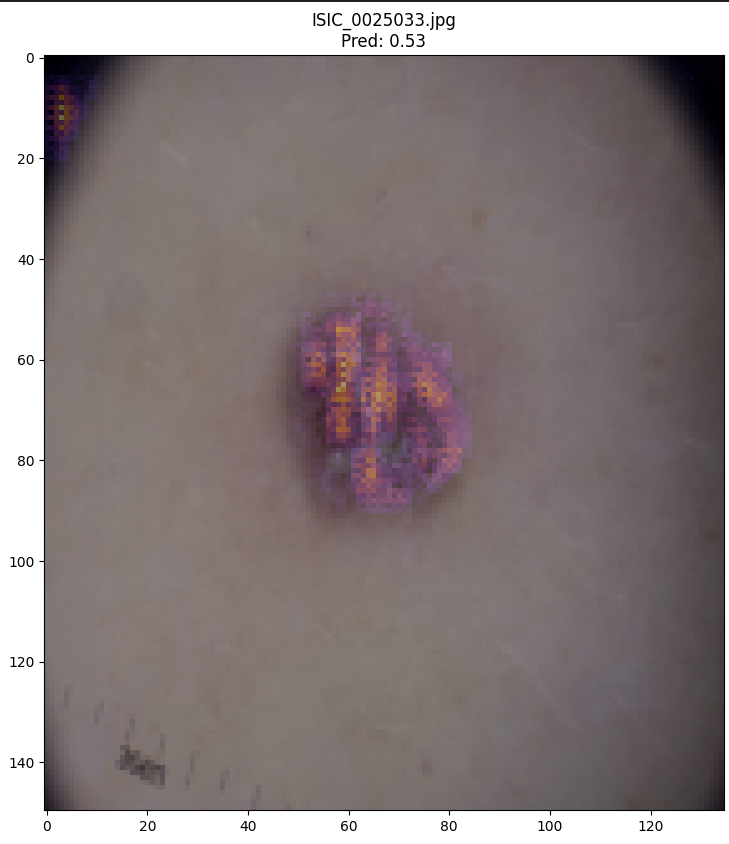
\includegraphics[width=0.5\textwidth]{images/ruler_classifier_saliency.png}
    \captionof{figure}{Saliency map from a ruler classifier that I trained during the project.}
    \label{fig:ruler_classifier_saliency_map}
\end{center}

This clearly shows the Clever Hans phenomenon in action. So, the Clever Hans phenomenon is very real, but just because it could occur, doesn't mean that it will in all cases.
\subsection{Are no models affected by the rulers?}
As mentioned multiple times, multiple other researches have been convinced that the models that 
they trained were using the rulers.
It is impossible for us to verify without access to their model.
There is a possibility that the model trained in this project is simply better in some way, making it not use the rulers.
I am however critical of that theory, though I cannot refute it completely.
During the project, I trained many models of varying architectures,
and in none of them I was able to find clear-cut evidence that the model was using the rulers.
Even though I tried, making my models biased was difficult, 
so for someone to train a model accidentally that is seems unlikely - but of course not impossible.

\subsection{How big of an impact can be expected from confounding elements?}
% I'm honestly not that happy with argument (this paragraph) - maybe I should just delete it
Obviously, there are a lot of other confounding elements that could introduce the Clever Hans effect on models trained 
skin lesion images than just the rulers studied in this report.
Figuring out if a given model was using one specific element, 
was in itself quite a difficult task, 
so, answering the generalized question about whether a given model is affected by any confounding element,
is very difficult, if not impossible.
We can, however, say something about the subset of confounding elements that are on purpose introduced by a doctor, 
such as adding a ruler, looking through a microscope or drawing next to a lesion.
Since they are added by a doctor, they can never provide more knowledge than that doctor already had.
Doctors, looking at the images, get precision that wary between $74\%$ and $84\%$\cite{multi-class-skin-lesion-hybrid}.
If we can construct algorithms significantly outperforming that (like the one trained in this project),
then model must at least have learned \textit{something}, that the doctors didn't already know.
That argument is of course very dependent on how the data is collected,
as, the argument doesn't hold if the doctor has other external knowledge not extracted from the image.

Another fact that puts an upper bound on the impact of confounding elements is that the model
is performing better on the segmented images than on the non-segmented ones.
If there really was a lot of information in the confounding elements around the lesion,
then we would expect the model to utilize that information and perform better on the non-segmented images.
It is of course possible that there is some artifact in the image, like the setting of the lighting or the type of camera used,
that the model is using but is not removed by the segmentation.
As mentioned before, the general problem of making sure that the model is using \textit{only} the information that we as 
the engineers deem \textit{relevant} is almost impossible.
The best way to do that in practice is to train the model on data that is collected in the same way,
as the data that it has to be used on.
In that way, it doesn't contain any information it is not allowed to use.

\subsection{Why are these results even relevant?}
One could argue that the fact that a given model does not seem to be using a specific element of the images it was trained on, 
is in itself not a very interesting finding.
The results I find interesting is not as much that the models are not using the element,
it is how difficult it was to argue.
Deep neural networks outperforms everything else in this field,
but we have no idea what they are doing and trying to figure it can be very difficult if not impossible.
So, these results should serve as a warning about how difficult it is to understand what deep neural networks are doing,
and not to make fast conclusions from just a saliency map showing some small highlighted area that fits your theory.

\section{Further research}
\subsection{Checking through the results using a binary classifier}
To simplify the research in this project, only a single model has been used - namely, one that was trained on the multi-class problem.
When doing analysis and metrics that is only possible with a binary classifier,
we simply translated the $7$ classes into two classes (malignant and benign).
It could change some results of the project if instead the model was trained directly on the binary problem.
For instance, a binary classifier might be more likely to look at a ruler as a sign of malignancy,
as it is a strong indicator of that, but not weak in distinguishing between different malignant classes.

\subsection{Could segmentation improve state-of-the-art}
In this project, we trained a model that was almost state-of-the-art.
We saw a clear improvement in the performance of the model on the segmented images,
so, it is possible that making a model that would beat state-of-the-art by simply adding a 
segmentation layer to the current state-of-the-art model.

\subsection{Making a standardized test}
The central problem, in this project, was to find out if the trained model was using the rulers in the images.
That problem was extra difficult because there was not a standardized way of testing if a model was using some possibly confounding element.
As it is a problem that can happen in many areas of machine learning,
developing a standardized test might make it easier to test if a model is using a given element.
Currently, the researchers working in the field just find some way to test themselves and draw a conclusion from that.

